\documentclass[]{coda-art}

\addbibresource{zalaczniki/bibliografia.bib}
\graphicspath{ {./images/} {./images/logo/} }


% ===== STRONA TYTUŁOWA =============================================

\pretitle{Ogród Księżycowych Kwiatków\vspace*{-0.5ex}}
\title{Dotknięci Miłością}
\author{\textbf{\emph{violacoda}}, dla \textbf{\emph{Moonflowers Collective}}}

\noticeversion{\today}{%
    Wersja alpha 0.1/23m05a}
{%
    \vspace*{-0.5ex}
    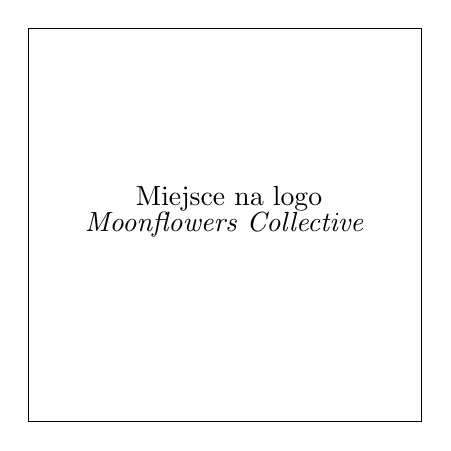
\begin{tikzpicture}
        \draw[draw=black] (0,0) rectangle (5,5)
        node[pos=.5] {\emph{Moonflowers Collective}}
        node[pos=.51,anchor=south] {Miejsce na logo};
    \end{tikzpicture} \\[0.7ex]
    \begin{flushleft}
        \hspace{2em} <moonflowers wkrótce!> \\[0.3ex] % \href{https://moonflowers.pl}{moonflowers.pl} \\
        \hspace{2em} \img{discord} \href{https://discord.com/invite/NFRSUEztRW}{Księżycowe Kwiatki} \\[0.3ex]
        \hspace{2em} \img{github} \href{https://github.com/violacoda/dotknieci-miloscia}{violacoda/dotknieci-miloscia}
    \end{flushleft}
}


\begin{document}

\titlecenter{%
    \vspace{1ex}\emphfont\it
    \begin{verse}[0.8\linewidth]
        \flagverse{\textcolor[HTML]{0466c8}{I:}}
        Nie pamiętam kiedy ostatni raz pozwoliłam sobie odpocząć \\
        \vin Gdy obrasta mnie księżycowych kwiatów pnącze \\
        Żyję hermetycznie, pochłonięta przez chorobliwość \\ 
        \vin Przez pryzmat której widzę i co na moich oczach rośnie

        \vspace*{-1ex}
        \flagverse{\textcolor[HTML]{9e2a2b}{E:}}
        Jesteśmy jednością rozbitą w binarność \\ 
        \vin Ja nie więcej jak gościem w Twojej domenie \\
        \vin I śmiercią zniekształconą przez Twoją projekcję \\
        Dotknięta nieśmiertelnością, aż zakwitniesz \\
        \vin Dopókiśmy rozbici nie doświadczymy śmierci \\
        \vin W inkluzji, ślepi na miłość z której się zrodziliśmy \\
        Spętani kwiatami ogrodu chorobliwości \\ 
        \vin Pod nocną kompozycją zakwitnijmy tańcząc \\
        \vin Do samozniszczenia nas obu, by znów stać się jednym
    \end{verse}
    \hfill {-- \textsc{violacoda}, \small\emph{Kwiaty Ogrodu Chorobliwości}}
}

\titleleft{
    \small Dokument udostępniono na licencji: \\[-0.5ex] 
    \footnotesize\sf\href{https://creativecommons.org/licenses/by/4.0/deed.pl}
    {CC\! BY\! 4.0\! --\! Creative\! Commons:\! Uznanie\! autorstwa}. \\[1.9ex] \rm\small
%
    Jesteśmy \emph{Moonflowers Collective}, społeczność artystycznych duszyczek kwitnących pięknie nocą, jak księżycowe kwiatki.
    \emph{Ipomoea alba}, te kwiaty są dla nas symbolem dualizmu Miłości i Chorobliwości. 
    W chorobliwej nocy i cierpieniu odnajdują Miłość, światło i uzdrowienie, aby zakwitnąć prawdziwym i unikatowym pięknem. \\[1.8ex]
%
    Współtworzymy kolektyw rannych uzdrowicieli.
    Miłość jest tym, co pozwala uzdrawiać. 
    Nauczamy więc jak cierpieć świadomie i jak siebie uzdrowić sztuką miłości.
    Wierzymy, że filozofia, psychologia, sztuka oraz miłość, tworzą najgłębszy dialog do zrozumienia ludzkiego istnienia. \\[1.8ex]
%
    Praktykujemy postawę i filozofię, gdzie nazywamy się \emph{Dotkniętymi} (cierpieniem, chorobliwością), więc \emph{Dotkniętymi Miłością}. 
    Aby nauczyć jak kochać siebie i innych, aby dotknąć ludzkie serca sztuką miłości.
}

\abstract{%
    Filozofia jest sposobem bycia, aktem życia, czyni sie ją w każdym momencie.
    Współczesna filozofia zapomniała o tej tradycji, a filozoficzny dyskurs wyprzedził filozofię jako postawę w życiu.
    Prawdziwa filozofia nie jest zlepkiem technicznego żargonu dla specjalistów, jest postawą istnienia w świecie, w ktorym praktykuje sie miłość w każdej chwili. 
    Jej celem jest przekształcenie całego życia jednostki, aby stać się najlepszą wersją siebie.
    Wcieleniem tego Ja jest wizja, z natury artysty jego największe i najpiękniejsze dzieło.
    W sztuce miłości zmiana Ja, zabicie ego, to opus magnum artysty, co wiąże doświadczenie śmierci z miłością pod postacią indywidualnej wizji.
    Mądrość nie sprawia, że coś po prostu wiemy; sprawia, że „jesteśmy” w inny sposób.
    Jesteśmy rannymi uzdrowicielami, Dotknięci Miłością.

    Archetyp rannego uzdrowiciela leży na dnie każdej szczerej formy uzdrawiania.
    Jej fundamentem jest budowanie głębokiej świadomości i zrozumienia własnego Ja oraz świata, w którym żyjemy.
    Dopóki czujemy się prześladowani, zgorzkniali i żywimy urazę do naszej rany, 
    i staramy się uciec od cierpienia, pozostajemy nieuchronnie z nią związani.
    Rana może Cię zniszczyć, albo obudzić.
    Uzdrowienie swego Ja jest sprawą indywidualną, która musi wypływać z psychiki, 
    aby istniało rozwiązanie problemu, czym jest dokładnie co termin indywiduacji implikuje.
    Sztuka miłości to przyjęcie własnej wizji i swojego istnienia za najwyższą formę miłości i indywidualnej ekspresji.
    To wymaga, aby spróbować pokochać własną chorobliwość i odważyć się rozszerzyć tą wizję, świadomie ją urzeczywistnić.
    Kochać jest trudne i brutalne.
    Ale co pozostaje nam poza tym, aby kochać?
    Wszyscy cierpimy wystarczająco, niepotrzebnie.
    I dostrzec światło w tym mroku.
    W chwili największej słabości, kochać to najtrudniejsze, co można zrobić.
    A tego, jak kochać, ma ten dokument nauczyć.
}

\maketitle

\subsection*{Struktura Dokumentu}
\emph{Akt} jest zbiorem niezależnych \emph{rozdziałów} podzielonych na \emph{części}, w których mogą znaleźć się \emph{medytacje} wyrażające przemyślane myśli na daną część rozprawy.
Dokument został podzielony na siedem aktów rozwijanych niezależnie od siebie:

\paragraph*{Akt I: Sztuka Miłości}\, --\, Fundament filozofii dotkniętych miłością, świadomość, istota cierpienia oraz praktyka sztuki miłości.

\paragraph*{Akt II: Rozwój Osobisty}\, --\, Rozprawy z intencją niesienia pomocy w indywidualnym rozwoju i rozwiązywaniu osobistych problemów.

\paragraph*{Akt III: Komunikacja i Relacje}\, --\, Zasady zdrowej komunikacji, zależności tożsamości i ego, oraz budowanie i utrzymywanie relacji międzyludzkich.

\paragraph*{Akt IV: Filozofia i Psychologia}\, --\, Przedstawienie oraz zinterpretowanie dzieł sztuki, teorii i praktyk filozoficznych oraz psychologicznych.

\paragraph*{Akt V: Natura i Nauka}\, --\, Zjawiska świata fizycznego w obserwacji i eksperymentacji, więc nauka oraz obcowanie z przyrodą.

\paragraph*{Akt VI: Ogród Księżycowych Kwiatków}\, --\, Dzieje i najważniejsze osobowości Moonflowers Collective, interpretacje i historia projektów społeczności.

\paragraph*{Akt VII: Źródła}\, --\, Biografie, biblioteczka, źródła do dalszego zgłębiania wiedzy oraz praktyczne wskazówki jak z nich korzystać.

\begin{multicols}{2}
    \subsection*{Warunki}
    Dokument \emph{Dotknięci Miłością} jest otwartym projektem oraz dziełem organizacji Moonflowers Collective.
    To projekt polegający na kolaboracyjnym pisaniu, jest efektem otwartej współpracy społeczności Księżycowych Kwiatków.

    Dostępność dzieła nie jest i nie będzie ograniczana w żaden sposób.
    Każdemu pozwala się go używać, modyfikować i powielać w całości lub części całkowicie za darmo, zgodnie z warunkami licencji CC BY 4.0.
    Jeżeli masz wątpliwości co do tego, co możesz zrobić z naszą pracą, zapytaj się społeczności.

    \subsection*{Bibliografia}
    Dzieła cytowane i wykorzystywane w naszej pracy znajdziesz w dołączonej do dokumentu \hyperref[zal:bibliografia]{bibliografii}.
    Odwołuj się do przypisów bibliograficznych w tekście w celu identyfikacji naszych źródeł.

    Inną rolę czyni \hyperref[akt:zrodla]{Akt VII: Źródła}, którego celem jest zgromadzenie zewnętrznych zasobów wiedzy,
    wraz z notatkami jak z nich korzystać, wprowadzić biografię ważnych osobowości 
    oraz utworzyć biblioteczkę, aby dopełnić wiedzę z danej dziedziny.
    Do niektórych zasobów będziemy odnosić się w trakcie lektury.
    Tam znajdziesz dodatkowe źródła dla swojej indywidualnej pracy nad sobą.
    \vspace*{-0.8em}

    \columnbreak

    \subsection*{Współudział}
    Niniejsze rozprawy powstają z udziałem społeczności na otwartej przestrzeni forum.
    Publikując u nas własne treści lub udzielając się w rozwoju istniejących, przyczyniasz się do rozwoju dokumentu.
    Już samo zaangażowanie na forum sprawi, że Twoje uczestnictwo zostanie zarejestrowane.
    Bardziej wymagające prace i inne formy zaangażowania wyróżnią Cię wśród współautorów.

    Projekt jest i będzie \textbf{otwarty}, zaangażować się w niego może każdy.
    Doceniamy w społeczności każdy szczery udział w naszych projektach.

    Każdy zaangażowany w rozwój tego dzieła znajdzie siebie wraz z formą swego udziału na liście \hyperref[zal:wspolautorzy]{współautorów}, dołączonej na końcu dokumentu.

    Pamiętaj, że jeśli nie chcesz być na liście współautorów, możesz zrzec się tego wpisu w każdym momencie.
    Możesz określić w jaki sposób chcesz, aby Ciebie wpisano, np. pseudonim albo z imienia i nazwiska.
    Gdy Cię wyróżniono, twoje sociale czy osobiste portfolio na liście współautorów również mogą się znaleźć.

    Na naszym forum jest wątek dedykowany sprawom organizacyjnym.
    Odwołaj się do niego, jeśli chcesz poruszyć temat Twojego uczestnictwa w projekcie.
    \vspace*{-0.8em}
\end{multicols}

\subsection*{Ostrzeżenie}
Niektóre porady tu zawarte mogą być niebezpieczne dla twojego zdrowia
psychicznego i fizycznego, jeśli zastosowane nieostrożnie.
Praca duchowa jest z natury ryzykowna i niebezpieczna, gdy niewłaściwie stosowana lub niezrozumiana.
Nasze nauki nie są właściwe dla ludzi z poważnymi zaburzeniami psychicznymi, takimi jak:
depresja samobójcza, schizofrenia, psychoza, zaburzenie afektywne dwubiegunowe, 
uzależnienie od narkotyków lub inne schorzenia medyczne albo psychiatryczne.
Rozwój osobisty i duchowość nie zastępują profesjonalnego leczenia takich schorzeń.
Jeżeli praca duchowa powoduje, że twoje życie rozpada się w niezdrowy sposób, 
przerwij tę pracę, aż twój umysł się ustabilizuje i będziesz bezpieczny.
Nasze nauki mogą zostać łatwo niezrozumiane i źle zastosowane.
Nic czego nauczamy, nie promuje samookaleczania, samobójstwa ani jakiejkolwiek formy przemocy.
Nigdy nie myl tych pojęć z duchowym przebudzeniem, gdy mowa o śmierci ego.
Musisz pamiętać, że słuchając i stosując te nauki jesteś w pełni odpowiedzialny 
za konsekwencje, jakie się z nimi wiążą.
To nie są porady medyczne ani psycho-terapeutyczne, nie jesteśmy licencjonowanymi terapeutami.
Zadbaj o swoje bezpieczeństwo i bądź ostrożny przy pracy nad sobą.



\twocolumn\tableofcontents
%\oddblankpage

\onecolumn\clearpage
\pagestyle{fancy}


% ===== AKT I -- SZTUKA MIŁOŚCI =====================================

\clearpage\thispagestyle{akt}

\part{Sztuka Miłości}
\label{sztuka}

Funkcją tych nauk jest pomóc Tobie pogłębić Twoje zrozumienie rzeczywistości i zredukować samooszukiwanie się.
Ich celem nie jest sprawić, byś uwierzył w to, w co my wierzymy, 
ale aby zmotywować Cię do podjęcia się głębokiego i osobistego badania nad naturą Umysłu i Rzeczywistości 
-- najgłębszego z możliwych.
Twoja praca tutaj nie polega na przyjmowaniu naszych przekonań i wierzeń, ale na kontemplacji.
Uważaj, aby nie traktować kontemplacji jako dodatkowej, irytującej pracy, do której zmuszamy Cię kiedy wolisz robić coś innego.
Delektuj się możliwością poznania i doświadczenia swojej Świadomości.
W przeciwnym razie po prostu wpadniesz w przekonania i ideologię, jak każdy inny głupiec.

Nikt inny jak Ty nie zrozumie lepiej Twoich potrzeb i wizji, w której sie realizujesz.
Poznaj swoją własną prawdę, ona jest w Tobie.
Musisz być świadomy o naturze chorobliwości, aby móc się od niej uwolnić.
Ta praca nie jest perfekcyjnie czysta.
Jest zepsuta przez ego.
Znajdziesz nieprawdziwość w naszej pracy.
I jeśli nie będziesz ostrożny, pochłoniesz w sobie naszą korupcję.
Zastanów się, jak poważne to jest.
Nasza praca jest jedynie tak czysta, na ile my, jako kolektyw, moglibyśmy być w chwili, gdy ją tworzono.
Nie jesteśmy perfekcyjnie czyści, choć chcielibyśmy być bardziej.
Robimy, co możemy, biorąc pod uwagę, 
że sami indywidualnie musimy zadbać o własne przetrwanie i próbować nauczyć siebie samych kochać.
W każdych naukach znajdziesz poważne błędy i niedopatrzenia, oto jak trudna jest ta praca.
Możemy stale ją udoskonalać, ale nigdy nie osiągniemy perfekcji -- zostaje nam więc pokochać ten proces.
Żadnej pozycji nie można uznać za bezpieczną, a my nie jesteśmy wyjątkiem.
Bądź ostrożny i myśl za siebie.
Podejdź do tego odpowiedzialnie.

Nie interesuje nas tutaj ideologia duchowa czy filozoficzna.
To, co Cię ratuje, to kontemplacja i osobiste badanie, w które dobrowolnie i z radością się angażujesz.
To oczyszcza Cię z wszystkich ludzkich bzdur i złudzeń.
Stąd bierze się prawda.
Twoja prawda nie pochodzi od nas, ani od nikogo innego niż Ty.
Jako ranny uzdrowiciel, dotknięty miłością, zamierzasz użyć własnego umysłu, aby się oczyścić, 
tak jak kulturysta wykorzystuje lata podnoszenia ciężarów, aby wyrzeźbić swoje ciało.
Żadna ideologia nie dodaje mięśni do ciała, tylko trening.
Celem kulturystyki nie jest osiągnięcie jakiegoś końcowego rezultatu, 
ale czerpanie przyjemności z całego procesu podnoszenia ciężarów.
Więc zakochaj się w podnoszeniu.
Zakochaj się w kontemplacji!
Jeżeli bierzesz na poważnie swój rozwój i swoje życie, będziesz to robić przez kolejne paredziesiąt lat.
Nie da się osiągnąć osobistej doskonałości bez pokochania procesu.
Przestań ścigać się do jakichś wyimaginowanych wyników.
Zwolnij i delektuj się procesem.
To jest nauka płynąca z naszej sztuki.
Nie jesteśmy tutaj, aby uczyć Cię w co należy wierzyć.
Nie musisz w nic wierzyć, wystarczy że włożysz pracę w siebie samego przez cały ten czas, jaki Ci został.

Jeżeli w jakimkolwiek momencie studiowania naszej pracy znajdziesz części, 
które według Ciebie hamują którąkolwiek z funkcji naszych nauk,
więc ich roli w twoim samorozwoju,
chcemy abyś zignorował te części i podążał za własną prawdą.
Bądź szczery ze sobą, to pozwoli Tobie poznać własną wizję.
Twoja wizja mówi Ci, czym jesteś i do czego jesteś zdolny.
Każdy ma to w sobie, to jest Miłością.
Poznanie, doświadczenie i urzeczywistnienie tej wizji ma miejsce na domenie sztuki miłości.
To fundament filozofii Dotkniętych Miłością.
Cały ten akt jest poświęcony sztuce, która ma nauczyć Cię kochać i wyostrzyć narzędzia, 
którymi będziesz pracował przez całe swoje życie, codziennie.
Nie tylko jako artysta, ale przede wszystkim jako człowiek.

\ornamentbreak

Do rozwinięcia.
\vin Potencjalne tematy do poruszenia:

Miłość (rozwinięcie) \\
Świat jest prosty \\
Świadomość \\
Prawda \\
Uczucia i emocjonalna inteligencja \\
Epistemologia \\
Metafizyka \\
Akceptacja i wybaczenie \\
Sztuka i indywidualna ekspresja; ESTETYKA \\
Skupienie \\
Obserwacja \\
Szczęście \\
Wolność \\
Strach. Dlaczego boimy się prawdy? \\
Cierpienie \\
Dualizm \\
Mądrość i intuicja \\
Umysł, psychologia i neurobiologia (lub w akcie Nauka) \\
Ambicja i Wizja \\
Kreatywność i Destruktywność \\
Czas i Miejsce -- teraźniejszość, tu i teraz \\
Cierpliwość. Dlaczego wartościowe rzeczy wymagają rozwoju w czasie (lub w akcie Rozwój Osobisty) \\
Zmiana i zrozumieć nietrwałość \\
Śmierć

\clearpage\subfile{1-sztuka/milosc}
\clearpage\subfile{1-sztuka/zmiana}



% ===== AKT II -- ROZWÓJ OSOBISTY ===================================

%\oddblankpage
\clearpage\thispagestyle{akt}

\part{Rozwój Osobisty}
\label{akt:rozwoj}

Wprowadzenie do napisania.

\vin Potencjalne tematy do poruszenia:

Zdrowe i niezdrowe nawyki \\
Produktywność i prokrastynacja \\
Stres i walka z nim \\
Życie w codzienności, zdrowy styl życia \\
Siłownia, sport i kalistenika \\
Minimalizm \\
Zdrowie w żywieniu i dieta \\
Dziennik, czyli twoja osobista domena \\
Etyka pracy i praca głęboka \\
Motywacja \\
Nauka, bycie samoukiem \\
Pasje i zainteresowania \\
Praktyka medytacji \\
Wystaw siebie na doświadczenia \\
Szkoła, studia, system edukacji \\
Zarządzanie finansami i biznes \\
Zarządzanie czasem i produktywność \\
Inwestycja w siebie \\
Umiejętność rozwiązywania problemów

\clearpage\subfile{1-sztuka/milosc}
\clearpage\subfile{1-sztuka/zmiana}



% ===== AKT III -- KOMUNIKACJA I RELACJE ============================

%\oddblankpage
\newpage\thispagestyle{akt}

\part{Komunikacja i Relacje}
\label{akt:komunikacja}

Wprowadzenie do napisania.

\vin Potencjalne tematy do poruszenia:

Ego i rozwój ego \\
Zasady zdrowej komunikacji \\
Komunikacja niewerbalna \\
Konstruktywna krytyka \\
Intencje \\
Empatia i wrażliwość \\
Przywiązanie i jak odpuścić \\
Trauma i wybaczenie \\
Samotność \\
Odwaga Bycia Nielubianym \\
Projekcja i manipulacja \\
Społeczeństwo \\
Przywództwo i liderzy \\
Rola współpracy \\
Oszustwa, scamy, nadużycia -- jak tego uniknąć? \\
Romantyczna Miłość, związki, randkowanie \\
Intymność emocjonalna \\
Poznawanie nowych ludzi, nowe kontakty \\
Przyjaciele. Jak zdobyć przyjaciół i utrzymywać przyjaźń \\
Płeć. Męskość i kobiecość \\
Świadoma polityka


\clearpage\subfile{1-sztuka/milosc}
\clearpage\subfile{1-sztuka/zmiana}



% ===== AKT IV -- FILOZOFIA I PSYCHOLOGIA ===========================

%\oddblankpage
\clearpage\thispagestyle{akt}

\part{Filozofia i Psychologia}
\label{akt:filozofia}

Wprowadzenie do napisania

\vin Potencjalne tematy do poruszenia:

Czym jest filozofia? Miłość do mądrości \\
Droga do samopoznania jest drogą przez piekło \\
Dynamika spiralna (Spiral Dynamics) \\
Mroczna filozofia Artura Schopenhauera \\
Zrozumieć nihilizm, doświadczenie pustki \\
Nadczłowiek Fryderyka Nietzsche \\
Cień, ranny psycholog, indywiduacja, psychologia analityczna Carla Junga \\
Psychologia mężczyzny-chłopca -- Puer Aeternus \\
Psychologia indywidualności Adlera (lub w akcie Komunikacja) \\
Psychologia rannego uzdrowiciela \\
Psychologia Szamana -- wewnętrzna podróż \\
Psychologia Alchemii -- wewnętrzne złoto \\
Psychologia oszusta -- trickster \\
Kosmiczny mistycyzm H.P. Lovecrafta \\
Kafkaesque -- mroczny świat i psychologia Franza Kafki \\
Ludzka kondycja ponad ludzką opinię \\
Kondycja ludzka w filozofii egzystencjalnej i egzystencjalna terapia: Jean-Paul Sartre, Martin Heidegger \\
Dialogi Platona, jak Sokrates i jego rozmówcy podejmują fundamentalne pytania dot. natury rzeczywistości, wartości i moralności \\
Psychologia transcendencji, czyli jak doświadczenia mistyczne i religijne wpływają na psychikę człowieka \\
Fenomenologia ducha \\
Stoicyzm, medytacje Marka Aureliusza \\
Dekadentyzm, chylenie się ku upadkowi


\clearpage\subfile{1-sztuka/milosc}
\clearpage\subfile{1-sztuka/zmiana}



% ===== AKT V -- NATURA I NAUKA =====================================

%\oddblankpage
\clearpage\thispagestyle{akt}

\part{Natura i Nauka}
\label{akt:natura}

Wprowadzenie do napisania.

\vin Potencjalne tematy do poruszenia: 

Księżycowe Kwiatki, lub ogólnie, nasze ulubione kwiatki \\
Astronomia i kosmologia, badania kosmiczne i eksploracja kosmosu \\
Architektura i Eudaimonia Machine \\
Zen i sztuka pielęgnowania ogrodu, jak filozofia Zen wpływa na podejście do natury i sztuki krajobrazowej \\
Neurobiologia i umysł \\
Teoria ewolucji \\
Ludzkie i społeczne oblicza zwierząt \\
Teologia natury i religijne podejście do przyrody \\
Przyroda i obcowanie z naturą


\clearpage\subfile{1-sztuka/milosc}
\clearpage\subfile{1-sztuka/zmiana}



% ===== AKT VI -- OGRÓD KSIĘŻYCOWYCH KWIATKÓW =======================

%\oddblankpage
\clearpage\thispagestyle{akt}

\part{Ogród Księżycowych Kwiatków}
\label{akt:ogrod}

Wprowadzenie do napisania.

\vin Potencjalne tematy do poruszenia: 

Geneza społeczności \\
Projekt moonflowers.pl \\
Najważniejsze osobowości w Moonflowers Collective \\
Projekty społeczności -- ich historia, organizacja, interpretacje jako dzieła \\
Przyszłość Moonflowers Collective

\clearpage\subfile{1-sztuka/milosc}
\clearpage\subfile{1-sztuka/zmiana}



% ===== AKT VII -- ŹRÓDŁA ===========================================

%\oddblankpage
\clearpage\thispagestyle{akt}

\part{Źródła}
\label{akt:zrodla}

Wprowadzenie do napisania.

\vin Potencjalne tematy do poruszenia: 

Wszelkie biografie ludzi historii, ich dzieła oraz nauki \\
Źródła osób trzecich do pogłębienia wiedzy na dane tematy, praktyczne wskazówki jak z nich korzystać

\clearpage\subfile{1-sztuka/milosc}
\clearpage\subfile{1-sztuka/zmiana}



% ===== ZAŁĄCZNIKI -- BIBLIOGRAFIA ==================================

\clearpage\pagestyle{plain}

\phantomsection
\addcontentsline{toc}{part}{BIBLIOGRAFIA}
\sectionmark{Bibliografia}

\section*{Bibliografia}
\label{zal:bibliografia}

\ornamentbreak

\printbibliography[heading=none]


% ===== ZAŁĄCZNIKI -- WSPÓŁAUTORZY ==================================

\clearpage\pagestyle{plain}

\phantomsection
\addcontentsline{toc}{part}{WSPÓŁAUTORZY}
\sectionmark{Współautorzy}

\section*{Współautorzy}
\label{zal:wspolautorzy}

\ornamentbreak

\subfile{zalaczniki/wspolautorzy}


\end{document}
